\section{レポート課題4}
\subsection{課題1}
リアプノフ指数の $r$ 依存性を示したグラフを描け。但し、初期値をランダムに与え、グラフの横軸は $1 〜 4$ 、縦軸は $-3 〜 1$ までの範囲にすること。 $r$ の刻み幅は、各自適切な値を設定すること。\\
画像:\\
\begin{figure}[htbp]
  \centering
  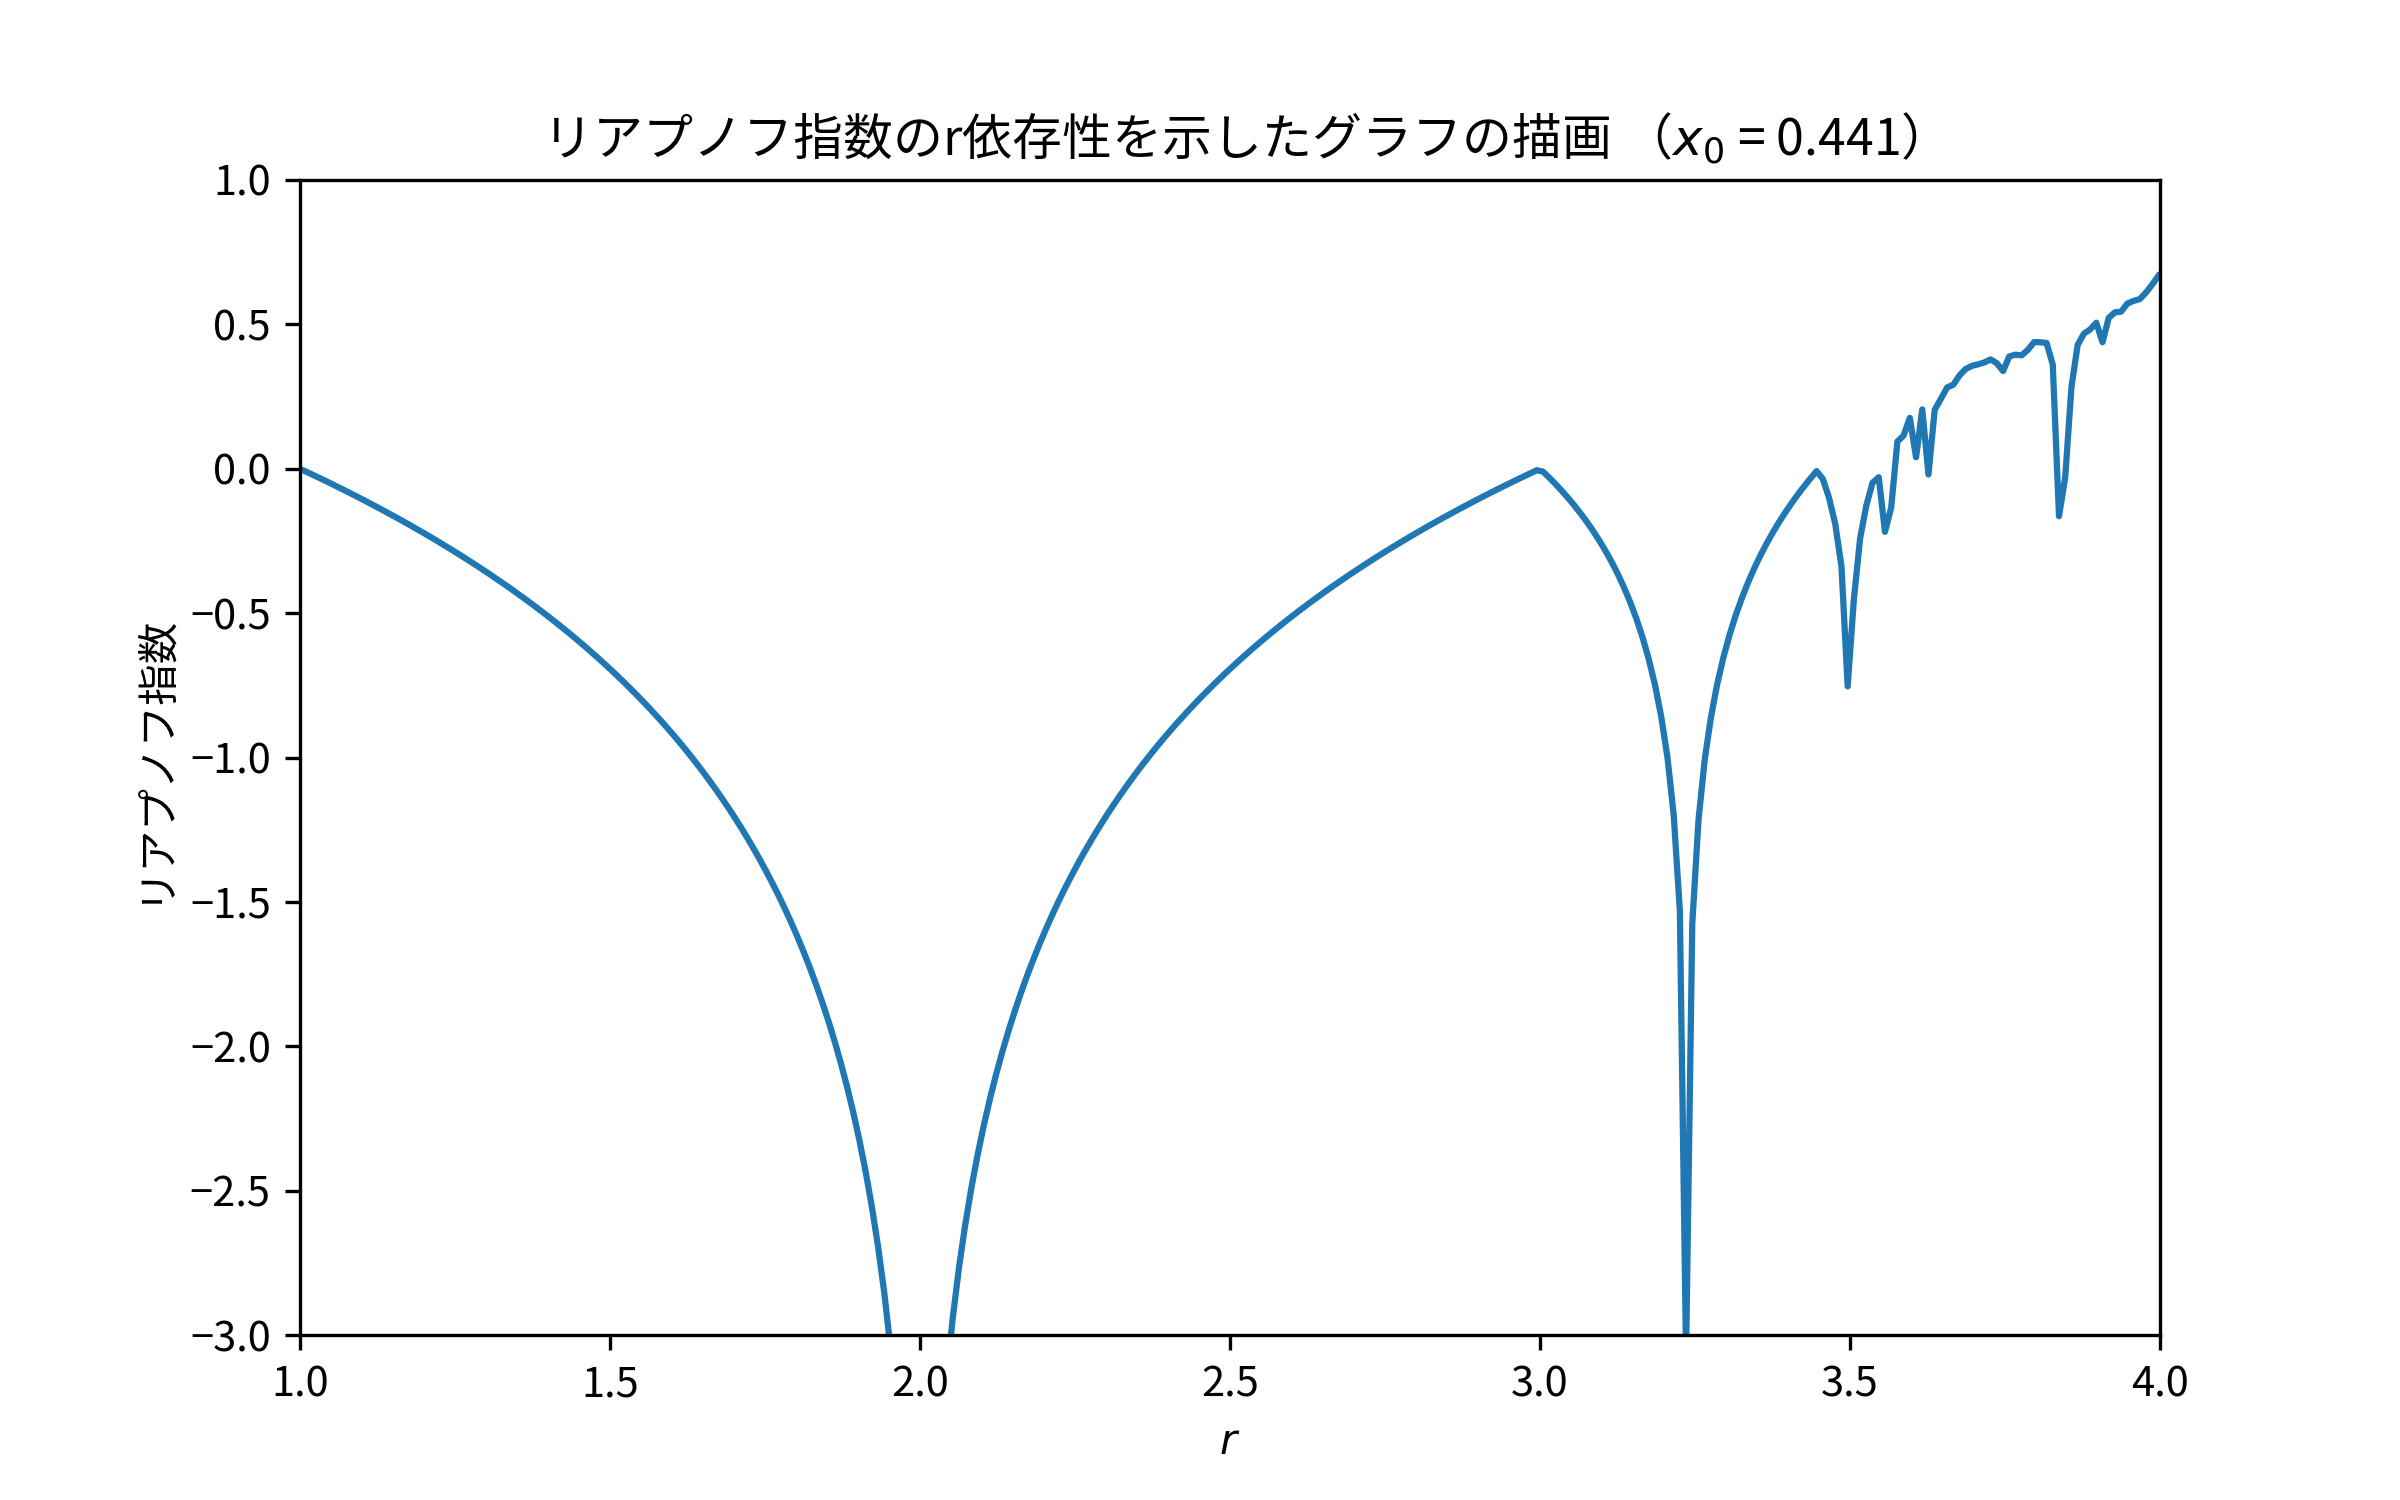
\includegraphics[keepaspectratio, scale=0.5]{images/Problem4/task4_1.png}
\end{figure}\\
結果:\\
$r$ の刻み幅は $0.0125$ ごとに設定しプロットした。この画像を見るとリアプノフ指数の値が負のときは、$r$ はなめらかに動いているため安定していると読み取れる。\\
考察:\\
これらの結果からリアプノフ指数の値が正のときは $r$ の細かい違いで大きな変化があることが予想される。この次の課題でより正の部分の挙動を見ることができるためこの考察が正しいかどうか調べていきたい。\\

\newpage
\subsection{課題2}
3周期の窓の領域でのリアプノフ指数の $r$ 依存性を示したグラフを描け。但し、初期値をランダムに与え、グラフの縦軸は $-1 〜 0.4$ までの範囲にすること。 $r$ の範囲および刻み幅は、各自適切な値を設定すること。
画像:\\
\begin{figure}[htbp]
  \centering
  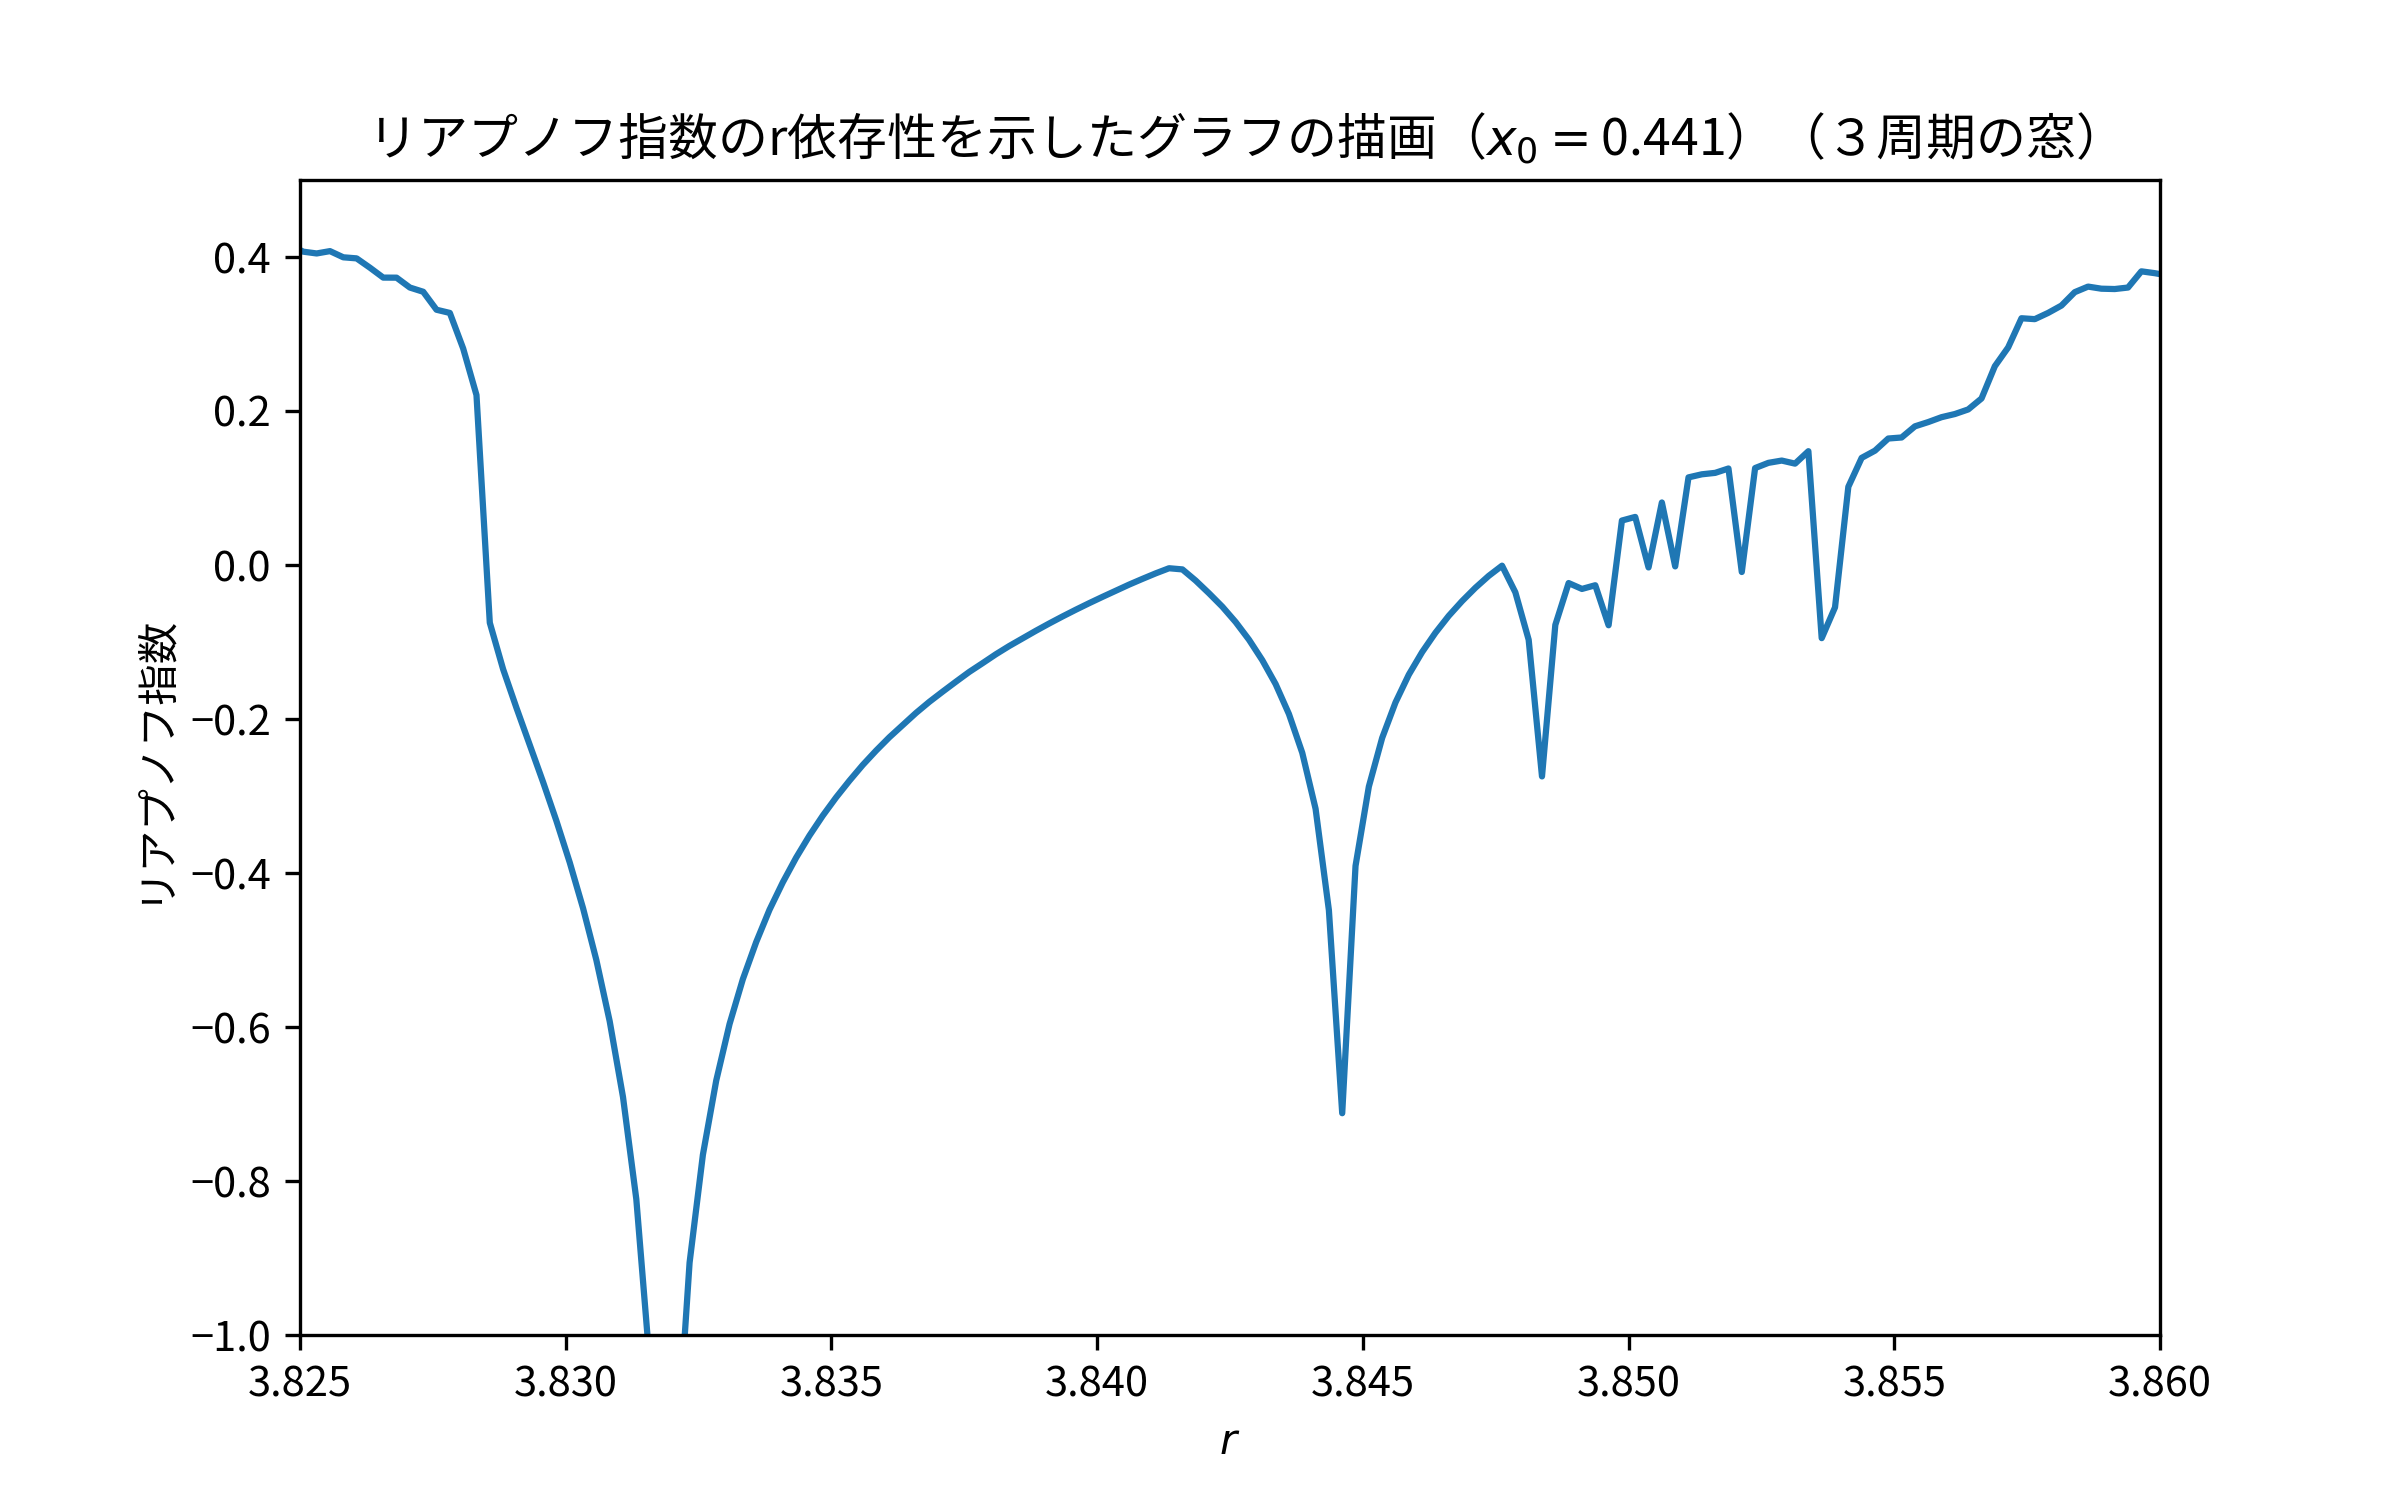
\includegraphics[keepaspectratio, scale=0.5]{images/Problem4/task4_2.png}
\end{figure}\\

結果:\\
$r$ の刻み幅は $0.00025$ で設定し、範囲は $[3.8, 3.9]$ で計算を行った。この画像から3周期の窓の領域ではおよそ3度ほど安定している範囲に入り、その後また不安定な挙動をすることが読み取れる。\\

考察:\\
これらの結果から、3周期の窓の領域の中に周期解を持つ範囲とカオスの特徴を持つ範囲に分けられると考察した。具体的には、リアプノフ指数が正の範囲でカオス、負の範囲で周期解を持つと考察した。また、課題1で言及していたリアプノフ指数の正負によっての違いだが、今回の課題2では非常に狭い範囲の中での $r$ とリアプノフ指数の値の関係性について画像で見ることができたので、リアプノフ指数の値が正のときに細かな違いで大きな変化があることがわかった。すなわちリアプノフ指数の値が正のときに初期値鋭敏性の特徴があると考察することができた。

\newpage
\subsection{課題3}
ロジスティック写像についてまとめ、これまでに出題された全て (4 回分 ) の結果について考察せよ。分量は A4 用紙 1 〜 4 枚程度を目安としてください。\\\\
 レポート課題1の考察は、ロジスティック写像は $r$ の値を変化させていくことで非周期性を満たすものと満たさないものがあると考察した。レポート課題1では初期値は $x_0 = 0.7$ に固定して $r$ の値によってどのような軌道になっていくかを比較した。それぞれの結果から、 $x_{n+1} = r(1 −x_n)x_n$ と $x_{n+1} = x_n$、 $x_0$ の位置関係と $r$ の値が収束、発散と関係していると考察した。\\
 レポート課題2の考察は、 $r = 3.86, r = 3.90$ のときは初期値 $x_0$ の小さい変化によって $x_{200}$ と $x_n (150 < n < 200)$ が大きく変化することが考察できる。レポート課題2では、初期値 $x_0$ の変化によって $x_{200}$ がどのようになっていくかを調べる問題になっていた。また、レポート課題2で比較した $r$ はレポート課題1と同様のものとなっている。レポート課題2の結果から非周期性を満たすかどうかは $r$ によって決まっていくことがより強く考察することができた。また、今回は初期値 $x_0$ を変化させていたので非周期性を満たすときの $x_{200}$ の挙動がどうなっていくか確認することができた。非周期性を満たすときの $x_{200}$ の値には規則性が見られることはなかった。これにより $r = 3.86, r = 3.90$ のときには初期値鋭敏性の要素が含まれていることが考察できた。初期値鋭敏性とは、初期状態での小さな差があると時間経過に応じて指数関数的にその差が増加するというカオスの条件のひとつである。\\
 レポート課題3は、添付している画像のランダムの値の他にもいくつかの値で課題1を実行してみたが、やはり $r = 1.50, r = 2.60, r = 3.20, r = 3.50$ のときはある値を反復し $r = 3.86, r = 3.90$ のときは値が定まることなく変化していた。これらの結果から $r = 3.86, r = 3.90$ のときはカオスの条件のひとつである非周期性が満たされていると考察することができる。また課題2の結果からこれらの結果から初期値 $x_0$ ではなく $r$ の値がカオスの条件と関係していると考察することができる。\\
 レポート課題4は、リアプノフ指数の値が正のときは $r$ の細かい違いで大きな変化があることが予想される。その考察の真相を明確にするために課題2を利用しさらに考察した。課題2から、3周期の窓の領域の中に周期解を持つ範囲とカオスの特徴を持つ範囲に分けられると考察した。具体的には、リアプノフ指数が正の範囲でカオス、負の範囲で周期解を持つと考察した。また、課題1で言及していたリアプノフ指数の正負によっての違いだが、今回の課題2では非常に狭い範囲の中での $r$ とリアプノフ指数の値の関係性について画像で見ることができたので、リアプノフ指数の値が正のときに細かな違いで大きな変化があることがわかった。すなわちリアプノフ指数の値が正のときに初期値鋭敏性の特徴があると考察することができた。\\
 これらの考察から、ロジスティック写像のカオスの状況は、 $r$ の値とリアプノフ指数の値によって左右されると考察できる。この考察をした理由はレポート課題3, 4での実行結果と考察が関係している。さらに、この考察を確認する方法として、レポート課題1, 2, 3でのプロットした画像がある。これらは、どの $r$ の値でカオスの条件になるか視覚的にわかりやすくしたものであり、また回が進むにつれ初期変動の影響をなくし、より鮮明にカオスかそうでないかを確認することができる。
\newpage
\begin{lstlisting}
  import matplotlib
  from matplotlib import pyplot as plt
  from matplotlib import colors
  import numpy as np
  from math import log
  from random import uniform
  # 日本語フォント用(Linux)
  matplotlib.rc('font', family='Noto Sans CJK JP')
  '''
  # 日本語フォント用(Windows)
  matplotlib.rc('font', family='MS Gothic')
  '''

  class Task4():

      def __init__(self) -> None:
          self.r = np.linspace(1, 5, 400, dtype=np.object)
          self.r2 = np.linspace(3.8, 3.9, 400, dtype=np.object)
          fig = plt.figure(figsize=(8, 10))
          self.ax1 = fig.add_subplot(2, 1, 1)
          self.ax2 = fig.add_subplot(2, 1, 2)
          self.ax1.grid(True)
          self.ax2.grid(True)
          self.x = uniform(0, 1)

      def f(self, r: float, x: float) -> float:
          "ロジスティック写像を返す関数(x の初期値はランダム)"
          return r * x * (1 - x)

      def f_prime(self, r: float, x: float) -> float:
          "ロジスティック写像の微分を返す関数(x の初期値はランダム)"
          return r * (1 - 2 * x)

      def calc_lambda(self, r: float) -> float:
          "乗数を計算する関数"
          lambda_sum = 0
          x_array = []
          cnt = 10000
          num = self.x

          for i in range(300):
              num = self.f(r, num)

          for i in range(cnt):
              x_array.append(num)
              num = self.f(r, num)

          for i in x_array:
              if self.f_prime(r, i) > 0:
                  lambda_sum += log(self.f_prime(r, i))
              else:
                  lambda_sum += log(-1 * self.f_prime(r, i))
          lambda_sum /= cnt
          return lambda_sum

      def problem1(self) -> None:
          "リアプノフ指数のr依存性を示したグラフの描画"
          lambda_array = []
          for i in self.r:
              lambda_array.append(self.calc_lambda(i))
          self.ax1.plot(self.r, lambda_array)
          self.ax1.set_title(
              "リアプノフ指数のr依存性を示したグラフの描画 ($x_0$ = {})".format(round(self.x, 3)))
          self.ax1.set_xlim(1, 4)
          self.ax1.set_xlabel('$r$')
          self.ax1.set_ylim(-3, 1)
          self.ax1.set_ylabel('リアプノフ指数')

      def problem2(self) -> None:
          "3周期の窓の領域でのリアプノフ指数のr依存性を示したグラフの描画"
          lambda_array = []
          for i in self.r2:
              lambda_array.append(self.calc_lambda(i))
          self.ax2.plot(self.r2, lambda_array)
          self.ax2.set_title(
              "リアプノフ指数のr依存性を示したグラフの描画($x_0 =${})(3周期の窓)".format(round(self.x, 3)))
          self.ax2.set_xlim(3.825, 3.86)
          self.ax2.set_xlabel('$r$')
          self.ax2.set_ylim(-1, 0.5)
          self.ax2.set_ylabel('リアプノフ指数')

      def save_fig(self):
          file_path = '複雑系科学演習/Week4/images/task4'
          plt.savefig(file_path, dpi=300)
          plt.show()

      def plot(self):
          self.problem1()
          self.problem2()
          self.save_fig()

  Lyapunov = Task4()
  Lyapunov.plot()
\end{lstlisting}